\documentclass{article}
\usepackage{amsmath, amssymb}
\usepackage{titlesec}
\usepackage[margin=1in]{geometry} % 1-inch margins
\usepackage{titling} % For custom title elements
\usepackage{tabularx} % For tables that fit within the page width
\usepackage{array}
\usepackage{pdflscape}   % Add this package for landscape
\usepackage{caption}     % Optional: For better caption formatting
\usepackage{float}
\usepackage{graphicx}    % If you're using \resizebox
\usepackage{cite}
\usepackage{rotating}
\usepackage{fancyhdr}
\usepackage{enumitem}
\usepackage{hyperref}

% Define a custom page style for landscape pages
\fancypagestyle{landscapeStyle}{
    \fancyhf{}
    \cfoot{\thepage}
    \renewcommand{\headrulewidth}{0pt}
    \renewcommand{\footrulewidth}{0pt}
}

\newcolumntype{Y}{>{\raggedright\arraybackslash}X}
% Define custom numbering format
\titleformat{\section}{\normalfont\Large\bfseries}{\thesection}{1em}{}
\titleformat{\subsection}{\normalfont\large\bfseries}{\thesubsection}{1em}{}
\titleformat{\subsubsection}{\normalfont\normalsize\bfseries}{\thesubsubsection}{1em}{}

% Customize the numbering scheme
\renewcommand\thesection{\Roman{section}}
\renewcommand\thesubsection{\Alph{subsection}}
\renewcommand\thesubsubsection{\roman{subsubsection}}

% Define subtitle command
\newcommand{\subtitle}[1]{%
  \posttitle{%
    \par\end{center}
    \begin{center}\large#1\end{center}
    \vskip0.5em}%
}

\pretitle{\begin{center}\LARGE\bfseries}
\posttitle{\par\end{center}\vskip 0.5em}
\preauthor{\begin{center}\large}
\postauthor{\end{center}}
\predate{\begin{center}\large}
\postdate{\end{center}}

\begin{document}

\title{Without Attraction, You've Got Nothing}

\author{}
\date{}
\maketitle

\section*{Foreword}
This paper is dedicated to the memory of Prof. Gian-Carlo Rota, whose work in Probability Theory has inspired me to think about the world in new ways. In 1993, Prof. Rota opened my eyes so that some months later I could appreciate the beauty and complexity of Prof. Steven Strogatz ideas. In 1993, neither one had any reason to take note of me as a student, but I will always remember them as the greatest of teachers.

\begin{quotation}
    [A] new unit in science is being formed that remains to be named. It will include the best of theoretical computer science, neurophysiology, molecular biology, psychology, and the mathematical theory of information. It will be important to name it properly. As the Latin proverb says, 'Nomen est omen.' We need to name it glamorously ... As is true in the early stages of any science, it's hard to tell the crackpots from the geniuses. They are minded together, as they were in the beginning days of physics when, for example, Kepler thought he could classify the distances of the planets from the sun by the lengths of the sides of the five regular solids inscribed in a sphere. Newton himself believed in magic... Everyone agrees that we must reform our programs at the Universities. But it is hard to change the sluggishness of an academic environment, and tension is building. We need imaginative new programs in mathematics;  \textit{we need daring departures that straddle mathematics, physics, and biology. For mathematical logicians most of all}. Witness the exodus of mathematical logicians out of their field into computer science. Thanks to logicians we have sophisticated programming languages and superior software. Computer science has become too important to be left to engineers. Fortunately, physicists and mathematicians are switching to computer and hardware design in great numbers. ...There is a ratio by which you can measure how good a mathematician is, and that is how many crackpot ideas he must have in order to have one good idea. If it's ten to one then he is a genius. ... An outstanding characteristic of mathematical talent is the ability to spot analogies. Another, one of the rarest, is the talent for applied mathematics, the talent for picking out of a maze of experimental data the two or three parameters that are relevant, and to discard irrelevant parameters. This is rare, because it is taught only at the shop level."
    \newline
    - \textbf{Gian-Carlo Rota},
    \textit{Mathematics, Philosophy, and Artificial Intelligence: a dialogue with Gian-Carlo Rota and David Sharp}, 1985\cite{Rota1985}
    \newline
    \newline
    Virtually all the major unsolved problems in science today have this intricate character. Consider the cascade of biochemical reactions in a single cell and their disruption when the cell turns cancerous; the booms and crashes of the stock market; the emergence of consciousness from the interplay of trillions of neurons in the brain; the origin of life from a meshwork of chemical reactions in the primordial soup. All these involve enormous numbers of players linked in complex webs. In every case, astonishing patterns emerge spontaneously. The richness of the world around us is due, in large part, to the miracle of self-organization.
    \newline
    ― \textbf{Steven H. Strogatz}, \textit{Sync: How Order Emerges From Chaos In the Universe, Nature, and Daily Life}\cite{Strogatz2003}
\end{quotation}

\newpage
\begin{abstract}
    This paper lays out an intuitive and formal arguments for scale-invariant Einsteinian physics that unify classical mechanics and Quantum Mechanics under Einstein's own 1905 tool-kit of ideas. By means of a logic proof that Quantum Mechanics is incomplete without quantum gravity Einstein's famous EPR argument is vindicated. The consequent mathematical derivation of Planck's Law under quantum gravity utilizes the purely discrete mathematics of Probability Theory to address the otherwise intractable Three-Body problem that results from applying gravity to the quantum scale.
    
    The prevailing understanding of Quantum Mechanics is called the Copenhagen interpretation, and it is predicated on the 400-year-old mathematical tool of calculus. Even by the physicists who ascribe to it, the Copenhagen interpretation defies any notion of common sense and reality. It maintains that a single entity can exist in a \textit{superposition} state—that is, "one thing can be in two places at once.” Famously, till the end, Einstein argued for reality as we know it and against the Copenhagen interpretation, but he has long been considered the loser in the debate. However, under the newer mathematics of Probability and Chaos Theory, this paper re-advances Einstein's now heretical discrete reality where one thing can only be in one place at one time.    
    
    To achieve a unification of Einstein's own work, we follow the ten lessons of Prof. Gian-Carlo Rota\cite{Rota1997}, father of modern combinatorics. This author attempts an intuitive explanation of Quantum Mechanics while providing a rigorous first principles reexamination of the contemporary masters Einstein, Poincar\'e, and Boltzmann. This author's limited bag of mathematical tricks are drawn from the latter two whose fields were in emergence while I was in college: Poincare's Chaos Theory \& Boltzmann's Probability Theory. 

    In a discrete reality, whether the scale is infinitessimally small like quanta or incomprehensibly big like galaxies, the introduction of gravity means the introduction of the chaotic Three-Body Problem - the problem that stumped Newton himself. As Poincar\'e showed, calculus offers no solution in Chaos. Thankfully though, using Boltzmann's balls-into-boxes Probability, "everything just works." With this bag of tricks, Einstein's macro-scale physics ideas from 1905 can be extended down to the quantum scale. Maybe this is what Prof. Rota meant by a "new unit in science" and is what Prof. Strogatz calls Sync. For my part, I can't explain why attraction exists, but I know that without it, you've got nothing. 
\end{abstract}
\tableofcontents
\newpage
\section*{Introduction: On a Heuristic Point of View about the Creation and Conversion of Light, Revisited}
\addcontentsline{toc}{section}{Introduction: On a Heuristic Point of View about the Creation and Conversion of Light, Revisited}
Perhaps the most famous problem in physics is the reconciliation of Quantum Mechanics with General Relativity. The former describes the behavior of particles at the smallest scales, while the latter governs the behavior of matter at the largest. The two theories are thought to be fundamentally incompatible, and the search for a unified theory that would bring gravity down to the quantum realm has been the holy grail of physics for over a century—but no headway has been made. Little did we know that the answer was right in front of us the whole time. This paper argues that the key to unifying Quantum Mechanics and General Relativity lies in the work of three contemporary geniuses of the turn of the 20th century: Albert Einstein, Henri Poincar\'e, and Ludwig Boltzmann. While the last century's worth of great physicists have scoured perplexing mathematics for clues to help them make history, we are now better served as mathematicians who scour perplexing history for clues to help us make great physics.

\begin{quote}
    “However, you have also understood correctly the disadvantage attached to a continuum. The question seems to me to be how one can formulate statements about a discontinuum without resorting to a continuum (space-time); the latter would have to be banished from the theory as an extra construction that is not justified by the essence of the problem and that corresponds to nothing ‘real.’ \textit{But for this we unfortunately are still lacking the mathematical form}. How much I have toiled in this direction already!!”

    \textbf{Albert Einstein}\textit{-1917 letter to Hans Walter Dällenbach}\cite{Einstein314}
    \end{quote}

The period spanning 1895 to 1905 was a remarkable decade for both mathematics and physics. 1905 is celebrated as Albert Einstein’s “Annus Mirabilis,” yielding groundbreaking work on the quantum nature of light\cite{EinsteinHeuristic}, the atomic nature of matter\cite{EinsteinBrownian}, special relativity frames of reference\cite{EinsteinRelativity}, and the mass-energy relationship\cite{EinsteinMassEnergy}. It is mind-boggling that atoms, quanta, energy, and the workings of gravity were uncovered in the same year by the same person, but even so, these were far from the only scientific miracles taking place. The decade leading up to 1905 also birthed fields that wouldn't be fully appreciated until well after the death of their fathers: Henri Poincar\'e's insights into the Three-Body problem, now the foundation of Chaos Theory, and Ludwig Boltzmann's organizing of atoms as "balls-into-boxes," the heart of Probability Theory. But, in 1905, Einstein's Relativity, Poincar\'e's Chaos, and Boltzmann's Probability were barely toddlers unknown to the world. Boltzmann passed in 1906 while the world still largely believed him wrong about the existence of atoms, Einstein's quantum theory was largely ignored for a decade, and the significance of chaos was unknown to even Poincar\'e in his lifetime.

The way their theories played together in their infancy is prescient of today's story: Boltzmann was a pioneer of the atomistic view of nature which Einstein proved; Poincar\'e formulated relativity first but Einstein gave it a natural framework; Poincar\'e pioneered the frameworks for dynamical systems, but Boltzmann's gave it applications and a computation method which was crucial to the development of Planck's Law; Boltzmann's work, which secretly underpinned Planck's Law, was the foundation for Einstein's 1905. However, the overlaps are probably more overshadowed by their separation. Today, their theories have matured only to find out that they were long-lost siblings whose lives were incomplete without the others. Together, we will retrace the story of how they lost each other and then jump forward to their reunion.

In the intervening century, the prevailing view of physicists is that reality has quite literally lost its meaning—Quantum Mechanics has demanded that "superposition" is real, that one thing can be in more than one place at a time, and that the moon does not exist when we are not looking at it. But in bringing the siblings back together, a new reality can emerge which is the original: one thing can be in only one place at one time. With this return of rationality also comes the notion that the laws of physics are the same everywhere, all the time, regardless of whether the scale is quantum or cosmological.

In this "scale-invariant" Einsteinian physics, particles are composed of small "balls" of energy, each of which individually act unpredictably in the same way their larger atom cousins do as per Einstein's 1905 Brownian motion. Similarly, in scale-invariant Einsteinian physics we would have definite-size Relativity frames which form "boxes" around the balls where gravity applies. The math of balls into boxes is Boltzmann's. Scale-invariant physics also mandates gravity at every scale, and with gravity comes the Three-Body problem and its chaos which are the province of Poincar\'e. The confounding result is that, out of the chaos of their countless, uncoordinated Brownian interactions within Relativity Frames, emerges Boltzmann's probabilistically characterizable "balls-into-boxes" order that is our observable physics.

Einstein's “On a Heuristic Point of View about the Creation and Conversion of Light,” introduced the concept of light quanta and first in the series that introduced the mass-energy equivalence formula $E=mc^2$, the existence of atoms with Brownian motion, and laid the foundations for quantum mechanics. Contemporaneously, Henri Poincar\'e, through his investigations into the gravitational Three-Body Problem, launched the field of Chaos Theory by describing dynamics that defied closed-form solutions\cite{Poincare1890}. At the very same time, Ludwig Boltzmann's statistical mechanics offered a wholly new approach to describing systems with many degrees of freedom. Yet, despite these advances and the subsequent emergence of digital computers that would ultimately prove crucial to realizing the potential of Chaos Theory, a critical question remains: can the insights of Einstein be unified across all scales, from the quantum realm to the cosmological, without resorting to paradoxical interpretations of reality? Calculus, the mathematical peer to the steam engine, was reaching its limits as a tool to describe the complexities of nature while a new era of computation, and the digital computer (peer to the jet), were still decades away. So, was Einstein correct to distrust the mathematics of his time? To complete his theories, were the new mathematical tools of his compatriots Poincar\'e and Boltzmann the missing pieces that would only come to full fruition well after all their passings?

This paper argues that the next leap forward in technological capabilities—particularly in building vastly more powerful “physics computers”—will stem not from the Copenhagen Interpretation of Quantum Mechanics championed by Einstein's philosophical nemesis Niels Bohr, but from Einstein himself, with an extension of his own ideas through the modern frameworks of discrete Probability Theory and Chaos Theory as implemented on digital computers. In other words, if Einstein is right, then the quantum computers currently being pursued by Google and others under Copenhagen assumptions simply won't work. Instead, using Einstein’s foundational ideas, it is possible that scalable, error-free “quantum supercomputing” architectures can be realized right now purely on digital platforms. By choosing the right physics—Einsteinian physics—we might immediately leap decades forward in computing capabilities.

To appreciate the significance of this claim, some historical and conceptual background is necessary. Nearly a century of debate surrounds the validity of Quantum Mechanics' idea of "superposition"—that one thing can be in two places at once. Formally, the debate is known as the Einstein-Podolsky-Rosen (EPR)\cite{EPR1935} paradox, and it has divided the physics community. At stake is the relationship between the two great pillars Einstein helped create: Quantum Mechanics and General Relativity. This debate has influenced every major innovation since the early 20th century, underpinning technologies from nuclear reactors to electronic computers and even guiding the financial engineering of the USD \$100 trillion derivatives market. On one side of the EPR debate stands Einstein, who believed that Quantum Mechanics was incomplete without the right mathematical tools. Without these tools, interpretations lead to bizarre scenarios: the moon existing only when observed, cats dead and alive at once, and “spooky action at a distance.” From Einstein’s viewpoint, no single physical object should occupy two places simultaneously—an intuitive, classical stance that he never abandoned. Opposing him are the Copenhagen interpretationists, including Niels Bohr and a litany of notable physicists, who insist that these counterintuitive features of Quantum Mechanics are indeed fundamental. Their stance has effectively won the last century’s worth of Nobel Prizes, asserting that “nonsense” must be accepted as reality, since no alternative explanation was readily available.

If genuinely error-free, scalable quantum computation emerges, the resolution of the EPR paradox—and, by extension, the question of whether Quantum Mechanics is complete or not—will shape the trajectory of science and industry for the coming century. The rewards would dwarf even the immense wealth and productivity gains of the past hundred years. But on what basis will quantum computing emerge? Will it be through the Copenhagen Interpretation, with its superposition and entanglement, or through a more intuitive, Einsteinian framework that eschews these paradoxical features? This paper argues that the latter path is not only possible but necessary for the next great leap in computational capabilities.

Before we dive into the formal proofs and discrete derivations needed to realize Einstein’s vision, consider Einstein’s own struggle to explain away the Copenhagen nonsense, expressed in his 1917 letter to Hans Walter Dällenbach \cite{Einstein314},
\begin{quote}
    "If the molecular interpretation of matter is the correct (practical) one, that is if a portion of the world must be represented as a finite number of moving points, then the continuum in modern theory contains much too multifarious possibilities. \textit{I also believe that this multifariousness is to blame for the founder of our tools of description of quantum theory...But for this we unfortunately are still lacking the mathematical form}. How much I have toiled in this direction already!!”"
\end{quote}

Modern quantum computing efforts largely ignore Einstein’s caution, accepting these multifarious extra constructions he opposed. The leading developers of Copenhagen-based quantum computing are designing them on the premise that they are literally sending computations into alternate universes. Yet, what if the mathematics Einstein sought—discrete, probabilistic, and inherently chaotic—can now be realized and, with it, simple common sense can be restored to physics?

This paper’s purpose is to show that such a mathematics exists and that it unites Quantum Mechanics and General Relativity into a single scale-invariant theory, without the counterintuitive leaps demanded by the Copenhagen Interpretation. Specifically, we will:
\begin{enumerate}
    \item Establish that Einstein’s skepticism about the completeness of Quantum Mechanics was justified, demonstrating how chaos and discrete probability can reproduce quantum phenomena without superposition.
    \item Show that the scale-invariance inherent in Einstein’s 1905 toolkit—quanta, Brownian motion, relativity frames, and $E=mc^2$—extends naturally into the quantum domain, linking macroscopic and microscopic physics under a single mathematical framework.
    \item Examine the explanatory power of this approach for previously unexplained phenomena, providing fresh insights into the fundamental nature of reality and the design of future computing architectures.
\end{enumerate}

In doing so, we are “revisiting” Einstein’s original heuristic viewpoint on the creation and conversion of light. By applying modern tools to Einstein’s old problem, we can finally realize the grand unification he sought but could not complete. The only superposition that will remain is a metaphorical one—a theory of physics which is both old and new at the same time. It is a scale-invariant Einsteinian physics that bridges the gap between the classical and quantum worlds, offering a path to the next century of great advances.

\section*{Quantum Gravity: Resolution of The EPR Paradox \& The Double Slit Experiment}
\addcontentsline{toc}{section}{Quantum Gravity: Resolution of The EPR Paradox \& The Double Slit Experiment}
\begin{quotation}
    "We choose to examine a phenomenon which is impossible, absolutely impossible, to explain in any classical way, and which has in it the heart of quantum mechanics. In reality, it contains the only mystery. We cannot make the mystery go away by “explaining” how it works. We will just tell you how it works. In telling you how it works we will have told you about the basic peculiarities of all quantum mechanics."
    \newline
    - \textbf{Richard Feynman}, \textit{The Feynman Lectures on Physics, Quantum Mechanics}\cite{FeynmanLectures}
\end{quotation}

Richard Feynman was a brilliant mind, a staunch defender of the Copenhagen Interpretation, and a renowned teacher. For these reasons we will borrow heavily from his explanations of the famous double-slit experiment (the DSE), the mystery "which as in it the heart of quantum mechanics."  

Before we dive in I think we should start with the conclusion because, if you lose hold of it, its likely this slippery subject will drag you in with no escape. In short, in the DSE it looks like a ball thrown at a wall can go through two slits in a wall simultaneously and even "interfere" with itself--that the ball can be in two places at once is the aforementioned "Copenhagen Interpretation." We will see that the Copenhagen Interpretation is premised on linearity, or that "balls move in straight lines." However, if you instead assume that balls move "non-linearly" in random, chaotic paths, then the DSE is no longer a mystery. This is the essence of the proof we will present.


\begin{figure}[H]
    \centering
    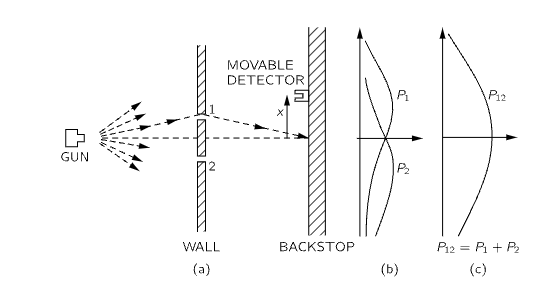
\includegraphics[width=0.8\textwidth]{images/Feynman_DSE_with_bullets.png}
    \caption{Feynman's Double Slit Experiment with bullets.}
    \label{fig:FeynmanDSEBullets}
\end{figure}

In this deceptively simple experiment, a single particle or "bullet" in Feynman's Figure \ref{fig:FeynmanDSEBullets}, like a photon or an electron, is fired at a barrier with two slits. As in Figure \ref{fig:FeynmanDSEBullets} one can imagine firing the bullets in many directions and what happens under various deflections but the end result after firing many many bullets adds-up to the distribution pattern in (c). But, if instead of firing bullets representing photons, actual photons are fired then what happens next defies common sense: you get the following distribution pattern which looks the same as sending water waves through the slits. This is the heart of the mystery of the DSE.:

\begin{figure}[H]
    \centering
    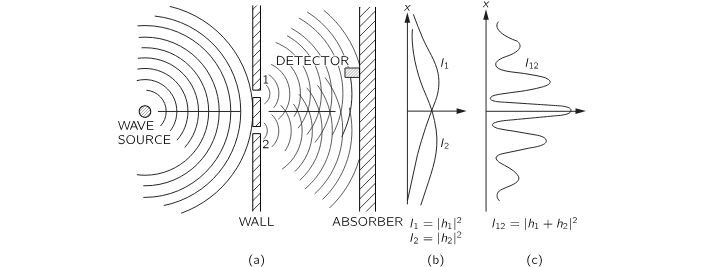
\includegraphics[width=0.8\textwidth]{images/Feynman_DSE_with_waves.png}
    \caption{Feynman's Double Slit Experiment with waves.}
    \label{fig:FeynmanDSEWaves}
\end{figure}


On the assumption particles move in straight lines, try as you might to come up with an explanation where the particle doesn't go through one slit or the other, you will be stumped and be forced to conclude that the particle passes through *both* at once, and when many particles are sent through the slits, they don't just make two lines on the detection screen, but a complex pattern of interference—as if they were waves, not discrete particles.  This pattern seems to suggest that each particle is somehow "aware" of the others, influencing each other's path, or that the particles are not particles at all but a wave moving through space.  According to the Copenhagen Interpretation, this bizarre behavior can only be explained by resorting to concepts like superposition and entanglement, ideas that Einstein himself found deeply unsettling.  Einstein, in his 1935 EPR paper, pushed back against this viewpoint, proposing a simple question: if our understanding of reality relies on such extraordinary postulates, is it not possible that we are missing something crucial in the underlying physics? Put simply, is Quantum Mechanics an incomplete theory? This is the riddle we must now address.

For this proof, we will introduce key concepts from Einstein's 1905 work—specifically Brownian motion and the principle of Relativity frames—arguing that these are essential missing pieces in the Quantum Mechanics puzzle. In our previous paper\cite{FRAQTL2024} (herein the FRAQTL paper), we demonstrated how gravity in a Relativity frame can induce Brownian motion and thus cause a particle to behave like a wave. The familiar visualization of Brownian motion often involves dropping balls at the top of a pegboard, which then form a bell curve as they descend. However, Brownian motion reveals something deeper: that atoms don't move in straight lines, but rather they stumble along a seemingly random, “drunkard’s walk” as they proceed towards their destination, swaying unpredictably from side to side. Now, imagine that particles such as photons also move this way. This insight connects back to the genius of Gian-Carlo Rota, whose work in Probability formalized many aspects of random motion.

\begin{figure}[H]
    \centering
    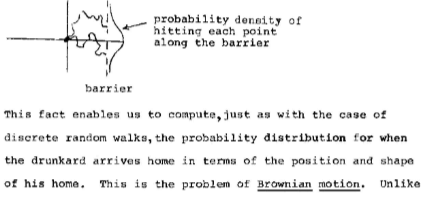
\includegraphics[width=0.8\textwidth]{images/brownian_Rota.png}
    \caption{Brownian Motion--Unpredictable path of two particles.}
    \label{fig:BrownianMotion}
\end{figure}

Think of the particles as those drunken walkers from Figure \ref{fig:BrownianMotion}, with their "home" representing the center of a Relativity frame. The squiggly lines represent the individual paths of two particles, each navigating a unique, random journey. Each particle, despite its chaotic path, tends toward its "home," building up a collective probability distribution—the bell curve—as particles arrive. As in Figure \ref{fig:BrownianMotion}, many particles starting from the same point will form a single bell curve, wave like, distribution. You might then imagine that if the particles were started a little bit apart from each from two different starting points, the bell curves would add-up, or "interfere", into a multi-humped wave interference curve...but you would then point to Figure \ref{fig:FeynmanDSEBullets} and say, then the interference pattern looks like (b) which adds up to (c), so you haven't explained anything. This is where the role of a finite Relativity frame comes in. If we imagine the drunken particles being in a box of some fixed size, say 10 drunken steps, where there is a "home" at each end, then every ten steps, once they get to the end of the box, they turn around and start over from wherever they happen to be in the box. From the particle's perspective this is the same as there being a slit every 10 steps and that slit happens to be wherever the particle ended up. So, they have some periodic motion to their random walk and the distributions keep adding up in complex ways.

There is no good way to show this in a static diagram but a good approximation is if you imagine that there is a "home" at each one of the concentric circle lines after the wall in Figure \ref{fig:FeynmanDSEWaves}! Mathematically, this is exactly how the fundamental wave equations are derived in the Fresnel diffraction integrals—the same equations that describe the DSE. The Fresnel integrals assume that *every point on a wave front acts as a new source of spherical waves (Huygens' Principle)*, and that these waves interfere with each other. Just as Fresnel assumed that every point on a wave front acts as a new source of spherical waves, each time a particle completes its 'drunkard's walk' within the box and is 'reflected' back, it effectively acts as a new source of Brownian motion, radiating a new probability distribution. This is the same as the particles in the box of Figure \ref{fig:BrownianMotion} starting a new path at each point along the wall when they reach home. Just as the new waves in the Fresnel Integral are omni-directional, the random restarts of the Brownian motion mean the particle can move in any direction. When the number "N" of particles is large, this looks like the Fresnel integrals and the distribution is as in Figure \ref{fig:FresnelDSE}. Imagine dropping a pebble into a pond (Brownian Motion). Now, imagine that after a short time, the edge of the ripple is *suddenly* changed to become the *center* of a new set of ripples that spreads out in all directions. These concentric circles are like the successive restarts of the Brownian motion when it reaches the end of its relativity frame. This is what causes the overall pattern.

\begin{figure}[H]
    \centering
    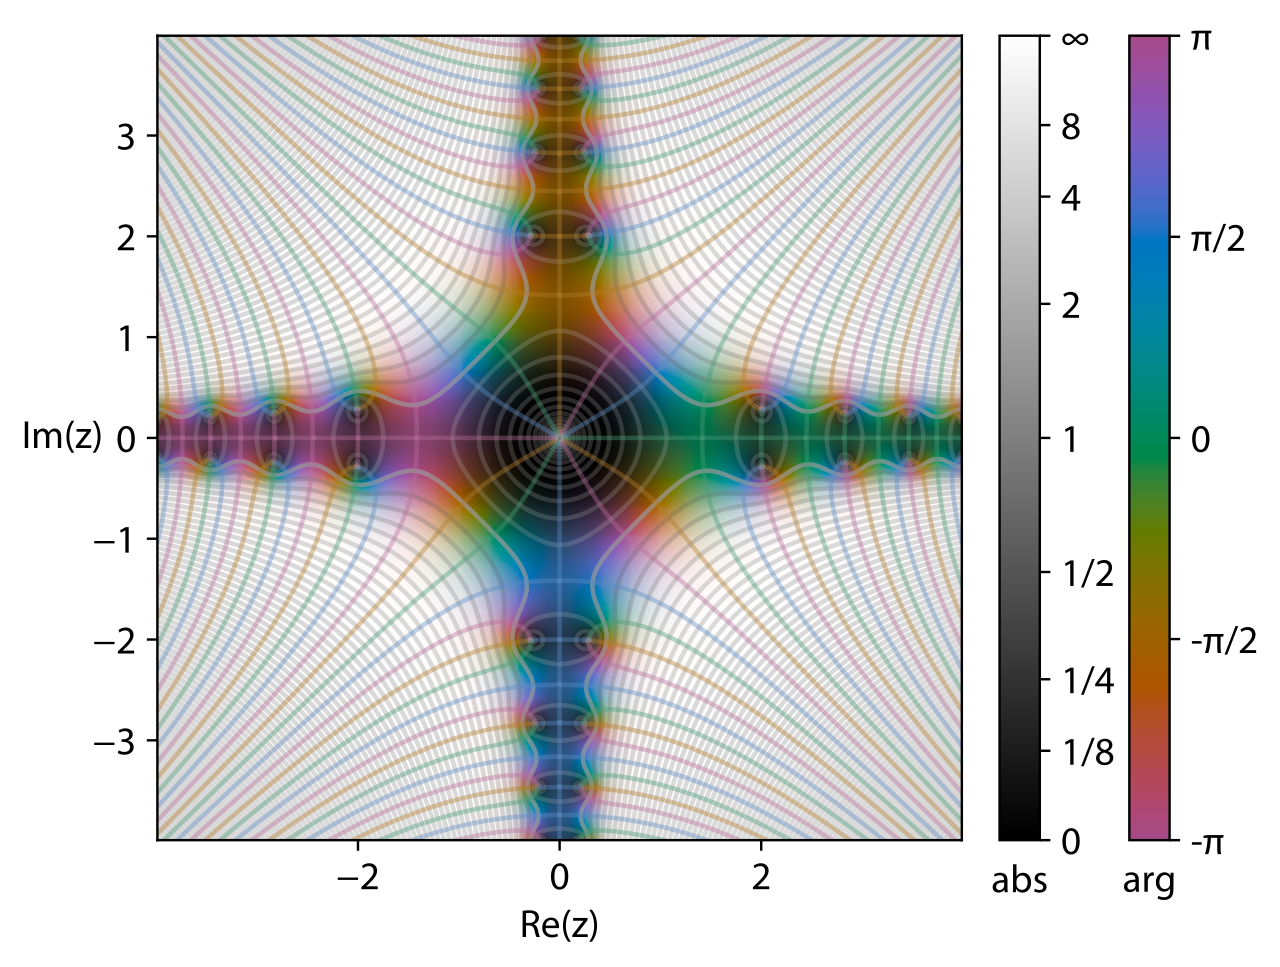
\includegraphics[width=0.8\textwidth]{images/Fresnel_integrals.png}
    \caption{Fresnel Diffraction Integrals. Image by Nschloe - Own work, CC BY-SA 4.0, \url{https://commons.wikimedia.org/w/index.php?curid=111944273}.}
    \label{fig:FresnelDSE}
\end{figure}

This simple yet powerful notion implies that the wave-particle duality isn't so mysterious after all; it's a natural consequence of the individual random walks of many particles combined with an attractive force bounding box that makes them periodic oscillators. In essence, the individual particles executing Brownian motion within a finite Relativity frame, when combined with the periodic restart, mimics the wave behavior described by Fresnel, where every point along a wavefront acts as a new source of spherical waves. Each particle makes its own independent choices, yet collectively, these random choices create a predictable, emergent, and complex wave-like patterns. The core of our argument is that these particles, like atoms, are not an abstract "wave function" or "field" that "collapses" when they are "measured"; they have a size and shape and they either collide with something or they don't.

Now, let's add another key player to our narrative: Henri Poincar\'e. In 1889, Poincar\'e made a profound discovery while studying the gravitational Three-Body Problem (e.g., the dynamics of three planets interacting via gravity). He showed that such systems cannot be solved with calculus, a tool that had long been the bedrock of physics. This discovery marked the birth of Chaos Theory, which reveals that, in seemingly random systems, there is a deterministic order so sensitive to initial conditions that it appears random. What's most compelling about chaos is that it can spontaneously produce order. Systems exhibiting chaos are often characterized by "strange attractors," stable patterns that emerge from the underlying deterministic chaos. Imagine this like a whirlpool in a stream: the water may move chaotically, but the whirlpool itself is a stable feature. So, without an attraction, there is no field of chaos, but with gravity (an attraction) comes both chaos and the resultant spontaneous order of strange attractors. Hopefully, the reader can now begin to see that the seemingly random behavior of a few particles can become a non-linear correlated behavior in a system with many particles.

In 1905, when Einstein had his "Annus Mirabilis," chaos was still a nascent idea, with strange attractors yet unknown. Instead of the framework that we are developing here, Einstein's contemporaries offered another explanation for the correlated behavior of particles in the DSE.  They argued that particles shared some initial "hidden information" at the start such that as they evolved toward a predetermined outcome —a kind of "you go left, I’ll go right" pact. These "local hidden variables" became a point of heated debate. Later, Bell's inequalities were interpreted to show that no theory with local hidden variables could reproduce the observed quantum correlations, seemingly reinforcing the Copenhagen view that superposition and entanglement were unavoidable.  However, these conclusions did not consider the crucial possibility that chaos and scale-invariant gravitational effects (quantum gravity) could generate the needed complexity and correlations without any hidden variables or faster-than-light signals. Modern studies demonstrate how systems like networks of oscillators can self-organize into correlated states (strange attractors) without any pre-shared information or signaling\cite{Watanabe-Strogatz1993}.

Let's take that lesson and apply it to quantum scales:  Consider that three or more bodies interacting gravitationally at the quantum level would induce chaotic dynamics. Through the principle of scale invariance, where the same rules apply at all scales, these chaotic dynamics would then apply universally but are attenuated by the size of the Relativity frame in which they act. At the quantum scale, particles will naturally fall into fractal-like distributions, creating stable statistical patterns—strange attractors—that mimic quantum probability distributions, all without hidden variables or superposition.

The logic of the proof below is simple: if adding quantum gravity completes Quantum Mechanics, then the resultant N-Body problem would introduce chaos that, via strange attractors, would naturally create the statistical signatures we associate with superposition and entanglement. If this were true, then Einstein’s intuition would be vindicated, and the Copenhagen Interpretation would prove to be an incomplete description of reality. Adding quantum gravity restores a more classical, albeit chaotic, explanation for quantum phenomena. To make this argument more than just a good story, we will now formalize it.

\subsubsection*{NB: On the Linearity of Paths vs. Linear "Betting Odds" in the Double Slit Experiment}
\addcontentsline{toc}{subsubsection}{NB: On the Linearity of Paths vs. Linear "Betting Odds" in the Double Slit Experiment}
Previously we spoke of linearity with respect to particles moving in a straight line like the bullets in Feynman's example-this was an oversimplification of linearity. A full mathematical treatment of linearity as it relates to the EPR paradox is not strictly needed for our proof below but it may still be intuitively helpful to discuss.  While it is beyond the scope of this paper to delve into the probabilities of gambling it may be interesting to the reader to peruse the introduction to Rota's Introduction to Probability Theory\cite{Rota1997} where he discusses Coin Tossing and the expactations of random walks - some very unexpected results occur from simple, fair coin tosses.\cite{Rota1985} 

Einstein, Podolsky, and Rosen (EPR) challenged the completeness of Quantum Mechanics because they thought that unexpected experimental results in the DSE must be the result of an incomplete understanding of physics, and not by some violation of physics as we know it. We can think of linear probabilities as the types of betting odds that happen at a casino or a horse track-people shouldn't be allowed to "beat the odds." In response to the EPR paradox, John Stewart Bell formulated his now-famous "Bell's Theorem", which derives a set of inequalities that must hold for any theory with linear correlations (i.e. "fair" betting odds). Imagine a horse-race betting site that sets "fair" odds for each horse based on standard assumptions. In this scenario, there are three main ways someone could cheat so that the final outcome doesn't match those odds. 
\begin{enumerate}
    \item \textbf{Non-locality:} the bettor receives the race result faster than the house's update (as though using a faster than light telephone signal) — analogous to “spooky action at a distance.”
    \item \textbf{Hidden variables:} the bettor starts the race with secret information the house doesn’t possess — like predetermined initial states for particles.
    \item \textbf{Reality isn’t fixed:} the bettor has a conspirator at the track who effectively \textit{decides} the race outcome in the bettor’s favor—meaning the “real” winner doesn’t exist independently until it’s reported.
\end{enumerate}
Bell’s inequality says that if your system is \textit{local} (no faster-than-light signals), \textit{realist} (the outcome exists in advance), and has \textit{linear} correlations, then you can’t systematically beat the odds. In essence, Bell formalized that if those assumptions are true then all relationships must be linear (with no extra "cheats").

However, Bell’s analysis assumes a \textit{linear} relationship to begin with, and it is that assumption that we choose to challenge in this paper. If the gambling system allows for \textit{non-linear} correlations—akin to reshaping how odds are calculated—then you could exceed those classic odds limits without resorting to any of the above “cheats.” In other words, you’d look like you were gaming the system under a linear model, but you wouldn’t actually be breaking locality or realism; you’d simply be using a different (non-linear) probability rule that Bell’s inequality does not address. Specifically, if your model has three properties--non-linearity, locality, and realism--then it is able to explain the Double Slit experiment without invoking concepts such as non-locality and superposition, and hence, we might conclude that Copenhagen based Quantum Mechanics is incomplete. 

Our logic proof below is premised on known behaviors of strange attractors in non-linear dynamic systems. While we believe non-linearity is the mechanism that lets particles "beat the odds," it might be that some other mechanism is at play and including this argument would unnecessarily complicate the proof.

\subsection*{Formal Proof: Quantum Gravity Completes Quantum Mechanics \& Resolves EPR Paradox}
\addcontentsline{toc}{subsection}{Formal Proof: Quantum Gravity Completes Quantum Mechanics \& Resolves EPR Paradox}
\textbf{Definitions:}
\begin{enumerate}
    \item \emph{Realism}: Physical properties exist independently of observation. The same rules apply across all scales.
    \item \emph{Scale Invariance}: The form of physical laws is invariant under changes in scale.
    \item \emph{No Local Hidden Variables}: No pre-encoded instructions or carried memory determine measurement outcomes.
    \item \emph{Locality (No Signaling)}: No information travels faster than light.
    \item \emph{Chaos and Strange Attractors}: Deterministic dynamics with sensitive dependence on initial conditions lead to self-organized, stable patterns without predefined states or signaling.
    \item \emph{Phenomena to Explain}: 
    \begin{itemize}
        \item $DSE$: The Double Slit Experiment pattern.
        \item $BELL$: Bell-type correlations.
    \end{itemize}
    \item $S(x)$: “Superposition/entanglement is strictly necessary for $x$.”
    \item $P(x)$: “A realistic, scale-invariant, chaotic, no-hidden-variable, local model (including quantum gravity) explains $x$.”
    \item $CI$: Copenhagen Interpretation.
    \item $QG$: Quantum Gravity (a scale-invariant gravitational interaction at quantum scales).
    \item $E(m)$: “Model $m$ is an incomplete understanding of Quantum Mechanics.”
\end{enumerate}

\textbf{Axioms:}
\begin{enumerate}
    \item \textbf{Realism and Scale Invariance Axiom}: The same physical principles (e.g., gravity, chaos) apply at all scales.
    \item \textbf{Locality Axiom}: $\forall$ spatially separated systems $(A_i,A_j)$, no superluminal communication influences outcomes.
    \item \textbf{No Shared Initial State Axiom}: Systems do not begin with pre-coordinated instructions determining all future measurements.
    \item \textbf{Chaos Axiom (3+ Body Quantum Gravity)}: With three or more particles interacting gravitationally at the quantum scale, deterministic rules plus sensitive dependence on initial conditions produce complex, fractal patterns (strange attractors).
\end{enumerate}

\subsubsection*{Proof By Contradiction}

\textbf{Goal}: To show that assuming superposition/entanglement as necessary leads to a contradiction if a chaotic, no-hidden-variable model with quantum gravity exists.

\textbf{Step 1 (Copenhagen Completeness Claim)}:
 Initially, the Copenhagen Interpretation (CI) is taken as complete if and only if superposition and/or entanglement are strictly necessary to explain both the Double Slit Experiment (DSE) and Bell-type correlations (BELL). Formally:
\[
S(DSE) \wedge S(BELL) \iff \neg E(CI),
\]
where $\neg E(CI)$ denotes that the CI is not incomplete (i.e., it is complete). This ensures that if we find a scenario where DSE and BELL can be explained without strict superposition/entanglement, CI cannot be considered complete.

\textbf{Step 2 (Alternative Model with Quantum Gravity)}:
Introduce a model $M = CI + QG$ that incorporates quantum gravity at small scales and is:
\begin{itemize}
    \item Realistic and Scale-Invariant.
    \item Local (no signaling).
    \item Without hidden variables (no pre-encoded outcomes).
    \item Chaotic: With three or more particles under quantum gravity, deterministic but highly sensitive initial conditions produce complex, fractal patterns (strange attractors).
\end{itemize}

If $M$ can reproduce the DSE and BELL phenomena without appealing to superposition/entanglement, we have:
\[
P(DSE): M \text{ explains DSE without } S(DSE),
\]
\[
P(BELL): M \text{ explains BELL without } S(BELL).
\]

\textbf{Step 3 (Chaos Implies No Local Hidden Variables)}:
By the Chaos Axiom, complex correlated outcomes emerge from deterministic chaos and gravitational interactions without any pre-encoded information. Thus, no local hidden variables are necessary. In other words, chaotic gravitational dynamics can yield complex, correlated patterns that mimic the statistical signatures of quantum phenomena without assuming any initial encoding of measurement outcomes.

\textbf{Step 4 (Implications of $P(x)$)}:
If $P(DSE)$ holds, we have:
\[
P(DSE) \implies \neg S(DSE).
\]
Similarly, if $P(BELL)$ holds:
\[
P(BELL) \implies \neg S(BELL).
\]

Combining both:
\[
P(DSE) \wedge P(BELL) \implies \neg S(DSE) \wedge \neg S(BELL).
\]

\textbf{Step 5 (Contradiction)}:
Recall from Step 1:
\[
S(DSE) \wedge S(BELL) \iff \neg E(CI).
\]
If $M$ exists and explains both DSE and BELL without superposition/entanglement, then:
\[
\neg S(DSE) \wedge \neg S(BELL).
\]

This directly contradicts the initial assumption:
\[
S(DSE) \wedge S(BELL).
\]

Since $S(DSE) \wedge S(BELL)$ was equivalent to $\neg E(CI)$, the contradiction shows that we cannot maintain that CI is complete if a $QG$ model explains the phenomena without strict superposition/entanglement. Hence, the initial assumption that CI is complete (dependent on superposition/entanglement being necessary) must be false.

\subsection*{Discussion: Intuition of Quantum Gravity Completing Quantum Mechanics}
\addcontentsline{toc}{subsection}{Discussion: Intuition of Quantum Gravity Completing Quantum Mechanics}

By positing a realistic, scale-invariant, local, chaotic model with quantum gravity that explains DSE and BELL correlations without superposition or entanglement, we have derived a logical contradiction with the assumption of CI's completeness. This supports the notion that CI may be incomplete. Rather than invoking superposition and entanglement, the necessary complexity and correlations can emerge naturally from chaotic gravitational dynamics. In subsequent sections, we will illustrate how this framework can also be used to derive Planck’s Law under quantum gravity, further strengthening the argument that Einstein’s intuition about a more complete, scale-invariant understanding of quantum phenomena may have been correct.

\section*{Derivation: Planck's Law Under Quantum Gravity \& Chaos}
\addcontentsline{toc}{section}{Derivation: Planck's Law Under Quantum Gravity}
Having shown that quantum gravity, chaos and scale-invariance can resolve the EPR paradox, a question naturally arises: can this new framework reproduce the foundational laws of physics? If the same logic applies across all scales, then it must also yield results that are consistent with what has been experimentally confirmed. We now turn our attention to a notoriously difficult problem in physics—the derivation of Planck's Law, the very equation that marked the birth of quantum theory. But where do we even begin? Perhaps by looking at what has already been ruled out and understanding how Planck himself arrived at his breakthrough.

\subsection*{Failed Correspondence, Or, "Calculus: The Wrong Tool For The Job"}
\addcontentsline{toc}{subsection}{Failed Correspondence, Or, "Calculus: The Wrong Tool For The Job"}
As we rigorously explored in the FRAQTL paper, calculus is an absolute impediment to describing a physics that includes Chaos Theory\cite{FRAQTL2024} since the very field of chaos was the result of Poincar\'e showing that gravitational N-Body problems have no closed-form (calculus) solution. But if calculus isn't the right tool, then what is? To find a different path forward, and to further reinforce that calculus is not the right tool for this problem, it's worthwhile to retrace some of the unsuccessful efforts of the 1980s and 90s when physicists attempted to apply the Copenhagen Interpretation to classical physics.

The "correspondence principle" of Niels Bohr, not surprisingly, states that Quantum Mechanics explains all other physics. Recall that the explicit assumption of Copenhagen is that the quantum realm is continuous and that calculus is its mathematics. In the 1980s and 90s, around the time Chaos Theory was gaining prominence, a related field called Quantum Chaos never quite took off. Michael Berry, one of the central figures in Quantum Chaos, penned a paper sub-titled "Is the Moon There When Somebody Looks?" and explained: "According to the correspondence principle, the classical world should emerge from the quantum world whenever Planck’s constant $h$ is negligible." Quantum Chaos was essentially an attempt to use the Copenhagen Interpretation to describe classical physics where gravity-induced chaos reigns (the N-Body problem). Instead of validating the correspondence principle, it served to prove the opposite; that the Copenhagen based Quantum Mechanics is fundamentally flawed \cite{Zurek1998}. The falsification of Copenhagen is semi-popularly known as "the problem with Hyperion" (a moon of Saturn). Noted quantum physicist, Sean Carroll, gives one of his typically elegant overviews:

\begin{quotation}
    "[Correspondence] is one of those vague but invaluable rules of thumb that was formulated by Niels Bohr back in the salad days of quantum mechanics. If it sounds a little hand-wavy, that’s because it is.
    \newline
    \newline
    The vagueness of the correspondence principle prods a careful physicist into formulating a more precise version, or perhaps coming up with counterexamples. And indeed, counterexamples exist: namely, when the classical predictions for the system in question are chaotic. \dots
    \newline
    \newline
    Some years ago, Wojciech Zurek and Juan Pablo Paz described a particularly interesting real-world example of such a system: Hyperion ... The orbit of Hyperion around Saturn is fairly predictable; happily, even for lumpy moons, the center of mass follows a smooth path. But the orientation of Hyperion, it turns out, is chaotic \dots
    \newline
    \newline
    So, in the real world, not only does this particular moon (of Saturn) exist when we’re not looking, it’s also in a pretty well-defined orientation \dots
    "\cite{CarrollHyperion}
\end{quotation}

Our objective is to find a mathematical framework for Quantum Mechanics upon which we can derive Planck's Law and other foundational relationships. As we just saw, the opposite could not be done—Quantum Chaos could not derive classical mechanics using Bohr's correspondence principle, the Copenhagen Interpretation, and calculus. This failure is a direct consequence of the foundation of Chaos Theory as formulated by Poincar\'e: chaos appears if gravity present, and chaos cannot be described by calculus. So, if calculus cannot describe systems where gravity appears, then how can it be the basis for a complete theory of physics?

It might seem that Quantum Chaos ruled out the possibility of Quantum Mechanics and classical physics from ever playing nicely together. However, in fact, all it did was rule out the Copenhagen Interpretation and its continuous assumptions. That is, if applying the Copenhagen Interpretation to classical physics fails, then the Copenhagen Interpretation is incomplete. This is the same conclusion we reached in the proof above and that proof was premised on a kind of "reverse-correspondence": that Chaos Theory can be applied to Quantum Mechanics and that doing so would make Quantum Mechanics complete.

\subsection*{Combinatorics: A Mathematical Form For A Discontinuum}
\addcontentsline{toc}{subsection}{Combinatorics \& The Three-Body Problem}
The Three-Body problem is a mythical beast of ornery mathematics, a problem that brought the great Newton himself to despair. With the idea of "reverse-correspondence" in mind, we opened a new door thinking it promising, but now we face the Three-Body monster head-on. If the goal is a theory of quantum gravity, should we try a "Chaotic Quantum Theory" of reverse-correspondence? The very fact that the Three-Body problem resists calculus should be a clear signal that we need a new mathematics, a mathematics capable of handling the discrete, the chaotic, and the discontinuous.

Letting history be our guide once more, we'll explore whether Planck's own derivation might give us a clue that will put this beast to sleep. Michael Fowler's wonderful recounting of Planck's work reveals: \cite{Fowler2008}

\begin{quotation}
    Planck was not impressed by [Boltzmann's] approach, since it implied that the Second Law was only statistical, only valid in the limit of large systems. However, he was fairly familiar with Boltzmann’s work — he’d taught it in some of his classes, to present all points of view. Planck wasn’t sure, though, that atoms and molecules even existed.

    Planck did this work by December 1900, in two intense months after learning the new experimental results and feeling he had to justify his curve that fit so well. But he only half believed it. After all, the first part of his derivation, identifying the energy of an oscillator with that in the radiation field, was purely classical: \textit{he’d assumed the emission and absorption of energy to be continuous}. Then, he suddenly changed the story, moving to a totally nonclassical concept, that the oscillators could only gain and lose energy in chunks, or quanta. (Incidentally, it didn’t occur to him that the radiation \textit{itself} might be in quanta: \textit{he saw this quantization purely as a property of the wall oscillators}.) As a result, although the exactness of his curve was widely admired, and it was the Birth of the Quantum Theory (with hindsight), no-one — including Planck — grasped this for several years!
\end{quotation}

After nearly a century of debate and attempts to unify the quantum and classical regimes, finding a theory of quantum gravity remains a formidable challenge. With that in mind, we will do as Planck did: we will use Boltzmann's methods, which, like all of combinatorics, is the mathematics of counting discrete possibilities, and we will blithely ignore the Three-Body beast... maybe it will simply go away. The approach here is to not simply "add more math" to a problem, but to ask what math is most appropriate for the job. If calculus, the math of the continuum, has failed, then what other mathematical tool should we use for a discontinuum?

The answer, it turns out, was already waiting for us in the work of Boltzmann—the mathematics of combinatorics. Combinatorics is fundamentally about counting the number of ways things can be arranged, the number of possibilities in a system. It is the mathematics of "balls-into-boxes", a discrete framework that naturally fits with a vision of a universe that is not continuous but granular, a universe made up of individual, countable quanta. While calculus deals with smooth curves and continuous change, combinatorics is perfectly suited to handle discrete objects and their interactions, and as such, it also suits our understanding of chaos.

By making the switch to a combinatorial perspective, we will bypass the difficulties inherent in the Three-Body problem, allowing us to proceed in a new, more tractable direction. Instead of attempting to solve complex differential equations, we will focus on counting the ways that energy can be distributed, a method that mirrors Planck's own approach when he first introduced the idea of quantization. Instead of asking what *can* happen, we will look at what is *most probable* to happen, just as Boltzmann did when he derived his famous H-Theorem. This move to combinatorics is not a random choice; it is a deliberate shift in our mathematical toolkit to match the discrete and discontinuous nature of reality itself, it is a move that we argue is necessary to bring gravity into quantum mechanics.

\subsubsection*{A Change In Perspective: Discrete \& Divisible Quanta:}
\addcontentsline{toc}{subsection}{A Change In Perspective: Discrete \& Divisible Quanta}
To recap, our objective is to bring gravity into Quantum Mechanics because we know that (Copenhagen based) Quantum Mechanics cannot be brought into classical gravity. In our previous proof we showed that chaos can resolve the EPR paradox, but we also know that the N-Body problem underlying chaos is incredibly difficult. To proceed, we are taking a page out of Planck's derivation of his own law, proceeding with Boltzmann's combinatorics to get over the Three-Body problem, and attempting a new approach to Quantum Mechanics that relies on discreteness.

Since combinatorics is the math of "balls-into-boxes," we have a new problem: what exactly are the balls, and what are the boxes? In Copenhagen Quantum Mechanics, particles are treated as point-like with no size and potentially occupying multiple places at once. Therefore, before we begin, we need to re-examine the foundational continuum assumption of the Copenhagen Interpretation and, once again, follow Einstein's intuition.

\begin{quotation}
    "Electrons (as points) would be final conditions (building blocks) in such a system. Do final building blocks exist at all?  Why are they all similar in size? Is it adequate to say: God in His wisdom has made them all the same size, each like the others, because He so wished? If it had suited Him, He could also have made them dissimilar." \cite{Einstein314}
\end{quotation}

In a discontinuum, every particle—like photons and electrons—must have a finite size and a definite position. Instead of treating photons as point-like (having no size), or as wave which is everywhere all at once, we will treat them each as a "box" having definite size and position. In fact, we'll even treat the quanta as divisible into smaller "energy unit" components that have no name in current physics (each a "ball"), with the understanding that these smaller components also possess the same properties. This is a departure from the current thinking, yet also a necessary step to get to a useful result.

Now, having changed our perspective we can add Einstein's 1905 toolkit, including quanta (discrete units which are divisible), Brownian motion (stochastic oscillators), Relativity frames, and the mass-energy relation $E=mc^2$. These subdividable quanta (frames) under stochastic motion and an attractive force will be shown to yield Planck’s Law.


\subsection*{A Blackbody Thought Experiment: The Blackbody Bus Station}
\addcontentsline{toc}{subsection}{A Blackbody Thought Experiment: The Blackbody Bus Station}

The discussion up to this point has seemed rather removed from an intuitive understanding of what is happening at the quantum level. Without such an intuitive understanding balls-into-boxes problems get very painful very quickly. Taking another page out of Einstein's book, let's try an accessible analogy. While Einstein often used a railway station as a conceptual tool, here we will consider a bustling `Blackbody Bus Station.'' Our aim is to understand the relationship between the number of passengers in the station and the fullness of buses when they depart. In this analogy, buses are colored according to how full they are: emptier buses appear red, and as they become more crowded, they transition through the spectrum towards blue.

At its core, the blackbody problem is about predicting the most probable colors of light emitted by a hot object. In more technical terms, color corresponds to the energy distribution of emitted light, also known as its spectral intensity. If an object is heated to 1000 K, will it emit more red light or more blue light? If it is heated further to 2000 K, how does the relative intensity of emitted red versus blue light change? Planck’s Law provides the quantitative relationship between temperature and spectral intensity.

To connect these ideas to our thought experiment, we will make parenthetical notes that relate station elements to their physical and mathematical counterparts. In the Blackbody Bus Station, the passengers (energy units) and bus drivers have been partying a bit too hard. As a result, they stagger about randomly, reflecting a stochastic random walk (Brownian motion). The passengers hop on and off buses (quanta) in seemingly chaotic ways, and the bus drivers, equally disoriented, swerve unpredictably (another manifestation of Brownian motion). All the while, the drivers shout at their passengers to move towards the center of the bus (an attractive force). A strict speed limit applies everywhere (Relativity frames), ensuring that passengers stumbling inside the bus, buses driving around the station, and even passengers wandering the station floor cannot exceed this universal speed (Lorentz invariance). Although their motion is random, the passengers and buses still tend to retain a memory of their previous direction (momentum in physics), which means our random walks have a certain persistence. Directional signs posted throughout the station encourage movement towards the center: passengers attempt to cluster near the bus’s center (quantum frame), while the buses, in turn, move towards the station’s center (station’s frame).

The fullness of a bus determines its color. Emptier buses correspond to lower-intensity, lower-frequency red light, while more crowded buses correspond to higher-intensity, higher-frequency blue light. The temperature of the station is related to the total number of passengers present. Just as a hotter oven radiates more blue light, a busier station tends to produce a greater proportion of fully loaded, bluer buses.

In summary:
\begin{itemize}
    \item \textbf{Bus Station:} The blackbody cavity from which energy (passengers) cannot easily escape until it finds its way onto a bus (quantum of light).
    \item \textbf{Buses:} Quanta of energy (like photons), each able to hold a certain number of energy units.
    \item \textbf{Passengers:} Individual energy units that behave like the smallest constituents of light, moving randomly.
    \item \textbf{Drunken Stumbling:} Stochastic random walk (Brownian motion). Both passengers and buses move randomly.
    \item \textbf{Speed Limit:} A universal limit on velocity (akin to the speed of light), ensuring a consistent relativistic frame for all movements.
    \item \textbf{Move-To-Center Signs:} An attractive force guiding energy units to cluster.
    \item \textbf{Bus Fullness and Frequency:} Spectral intensity. Fuller buses emit higher-frequency (bluer) light.
    \item \textbf{Temperature:} The total number of passengers. More passengers correspond to higher temperature, analogous to a hotter blackbody radiating more intense, bluer light.
\end{itemize}


\subsection*{Quantum Gravity, Balls Into Boxes Combinatorics, \& Chaos Strange Attractors}
\addcontentsline{toc}{subsection}{Derivation of Planck's Law \& Strange Attractors}

The key idea is that when energy is quantized into discrete units (like "balls") and placed into modes or states (like "boxes"), the distribution of these units can be understood purely combinatorially. When combined with an attractive force at the quantum scale—analogous to quantum gravity—this leads to stable configurations that yield the well-known Planck distribution without invoking superposition or other paradoxical notions.

\subsubsection*{From Chaos to Stable Quanta: Strange Attractors as Boxes}

Consider a blackbody cavity analogous to a "bus station" filled with many energy quanta ("buses") and discrete energy units ("passengers"). The energy units move randomly (Brownian motion) under a subtle attractive force—akin to a scale-invariant gravity at the quantum level. This force ensures that the quanta form stable "boxes" that can hold a certain number of energy units. In a chaotic, multi-body gravitational system, these stable configurations are like "strange attractors," fractal-like steady states that arise from deterministic chaos.

The presence of an attractive force is crucial: it prevents energy units from dispersing arbitrarily and ensures that stable states (modes) form. In essence, energy units cluster into quanta due to this attractive force, and we can count the probability distributions of energy among these modes using basic combinatorics. This approach turns what is an intractable non-linear dynamics continuous integral problem into an approachable, discrete counting problem.

\subsubsection*{Combinatorial Counting: Balls into Boxes}

We start by modeling the distribution of $M$ indistinguishable energy units (balls) among $N$ distinguishable modes (boxes). The number of ways to do this is given by the combinatorial formula:
\[
W = \binom{N+M-1}{M} = \frac{(N+M-1)!}{M!(N-1)!}.
\]
This formula counts the number of microstates (configurations) of energy distribution.

\subsubsection*{Increasing Temperature: Entropy and Stirling’s Approximation}
In our bus station analogy, increasing temperature corresponds to adding more passengers. Our initial task was to formulate the relationship between the color of departing buses and the total number of passengers in the station. Another way to phrase this is to ask how passengers will distribute themselves among the buses as the station gets busier. In thermodynamics which deals with atoms (much, much larger than quanta) there is a concept of entropy which relates how energy gets distributed. Why entropy should apply at the quantum scale isn't obvious unless quanta (our buses) are made up of smaller energy units (our passengers), however, since that is our assumption it makes sense to use the entropy relationship now. In thermodynamics our buses would be called "microstates" and the different passenger counts of buses are called "modes", so we will use that terminology interchangeably.
\newline

The entropy $S$ is related to the number of microstates by Boltzmann’s relation:
\[
S = k_B \ln(W).
\]
\newline
When $N$ and $M$ are large, we apply Stirling’s approximation:
\[
\ln(n!) \approx n \ln(n) - n.
\]
Using this approximation on $W$, we find a simpler expression for $S$:
\[
S \approx k_B \left[ (N+M)\ln(N+M) - N\ln(N) - M\ln(M)\right].
\]
\newline
Interpreting this entropy combinatorially reveals that the most probable distribution of energy among modes emerges naturally from counting arguments. The complicated integrals from the classical derivation of Planck’s Law are replaced here by discrete, combinatorial reasoning.

\subsubsection*{Relating Entropy to Temperature}
Returning now to the question of "what happens to the color of the buses as the station gets busier," we can ask this question mathematically by looking at the impact of adding a small number of passengers to the station  (i.e. we will take the derivative). Thermodynamics links temperature $T$ to entropy $S$ via:
\[
\frac{1}{T} = \frac{dS}{dU}
\]
where $U$ is the total energy. Differentiating the combinatorial form of $S$ with respect to $U$ and solving for $U$ as a function of $T$ yields a Bose-Einstein-like distribution. Identifying the quantum of energy in each mode as $hf$ (where $h$ is Planck’s constant and $f$ is frequency), we arrive at:
\[
\frac{U}{N} = \frac{hf}{e^{\frac{hf}{k_B T}} - 1}.
\]
\newline
This is the average energy per mode at frequency $f$ and temperature $T$, matching the quantum-statistical form known from standard quantum theory—but derived here from combinatorial logic and an underlying attractive force.

\subsubsection*{Density of States and Planck’s Law}

To obtain the full Planck’s Law, we multiply the average mode energy by the density of states $g(f)$. In a three-dimensional cavity:
\[
g(f) = \frac{8\pi f^2}{c^3}.
\]
\newline
Thus, the spectral energy density is:
\[
\rho(f,T) = g(f)\frac{U}{N} = \frac{8\pi h f^3}{c^3} \frac{1}{e^{\frac{hf}{k_B T}} - 1}.
\]
\newline
This is the celebrated Planck’s Law, now derived without invoking superposition or local hidden variables. Instead, we used:
\begin{itemize}[nosep]
    \item \textbf{Discrete Quanta:} Energy units placed in modes.
    \item \textbf{Combinatorics:} Counting microstates (balls into boxes).
    \item \textbf{Stirling’s Approximation:} Simplifying the factorial expressions.
    \item \textbf{Chaos \& Attraction (Quantum Gravity):} Ensuring stable, discrete modes form from chaotic dynamics.
    \item \textbf{Scale Invariance:} The same logic holds at all scales, from the quantum to the cosmological.
\end{itemize}
\subsubsection*{Connecting Back to Quantum Gravity and Chaos}

The crucial insight is that introducing a scale-invariant attractive force (i.e., a form of quantum gravity) allows for stable, discrete quantum states. The N-Body chaos becomes ordered into "strange attractors," each attractor acting like a stable "box" that can hold integer multiples of $hf$ energy units. The complex dynamical system is thus reduced to a combinatorial counting problem, revealing the Planck distribution naturally.

In essence:
\begin{itemize}[nosep]
    \item Chaos ensures complexity without hidden variables.
    \item Attraction ensures stable states.
    \item Combinatorics and scale invariance do the mathematical heavy lifting.
\end{itemize}

This viewpoint not only resolves paradoxes like EPR without the need for superposition but also shows that Einstein’s intuition about Quantum Mechanics being incomplete was correct. By incorporating quantum gravity and chaos, the full picture emerges, and the strange attractors at the quantum scale explain quantum statistics straightforwardly.


\subsection*{Why Attraction is Essential: Creating Stable Quanta}

Without the attractive force, energy units would never settle into discrete quanta. They would remain scattered, and the problem would remain intractably complex, akin to trying to solve an N-Body gravitational problem with no simplifying assumptions. The presence of quantum gravity at small scales provides a universal attractor, ensuring energy units cluster into stable configurations that can be enumerated. From this counting emerges the Bose-Einstein-like statistics that underlie Planck’s distribution.

In essence, \emph{There is Nothing Without Attraction}. This force molds the chaotic landscape of random walkers into stable boxes whose occupancies we can count. The result is a derivation that is as combinatorially straightforward as distributing people onto buses.

\subsection*{Scale Invariance and the Emergence of Planck’s Law}

Because this approach is scale-invariant, the same combinatorial reasoning applies at all levels. Zooming out, the differences between quantum and classical scales vanish in the logic of counting. At the smallest scales, quantum gravity ensures that energy units settle into stable attractors, just as at larger scales gravitational wells organize matter into stars and galaxies. This self-similarity of nature across scales—fractal in spirit—allows us to derive fundamental quantum laws from a discrete, combinatorial viewpoint.

When we follow the combinatorial steps in detail (see addendum), we find the well-known Planck’s Law formula. No continuous integrals or calculus-based derivations are strictly necessary, only careful counting of states and the recognition that a scale-invariant attractive force provides the stable "boxes" required to define those states. Thus, the celebrated formula:
\[
\rho(f,T) = \frac{8 \pi h f^3}{c^3} \frac{1}{e^{\frac{hf}{k_B T}} - 1}
\]
emerges from a logic chain grounded in chaos, scale invariance, quantum gravity-induced attractors, and combinatorial counting.

\subsection*{Combinatorics Addendum: Detailed Steps}

For those interested in the full derivation steps—from starting with raw combinatorial expressions (balls into boxes) to applying Stirling’s approximation and connecting the discrete results to the continuous limits known in classical physics—the addendum provides a thorough walk-through. At each step, the scale-invariant attractive force and the resulting stable attractors (our "boxes") play a crucial role, transforming a seemingly intractable N-Body gravitational problem into a manageable combinatorial puzzle. This detailed combinatorial path to Planck’s Law demonstrates that, with the right conceptual tools, Einstein’s original quantum insights can be integrated coherently with gravity and Chaos Theory, eliminating the need for paradoxical assumptions in Quantum Mechanics.

\section*{There is Nothing Without Attraction: Scale-Invariant Attractive Force}
\addcontentsline{toc}{section}{There is Nothing Without Attraction: Scale-Invariant Attractive Force}

In order to bring gravity into Quantum Mechanics and possibly complete the theory we had two approaches to choose from-calculus or discrete mathematics. Recalling that the N-Body problem, involving three or more bodies attracted to one another, is famously resistant to calculus solutions, we ruled calculus out as a mathematical form that Einstein would have sought. Instead, we found that introducing a scale-invariant attractive force gives us stable configurations of quanta so it transforms the problem into one of counting—effectively turning the complex dynamics into a balls-into-boxes scenario. Attraction ensures that the energy units form coherent quanta (our “boxes”), making a combinatorial approach feasible.

Without attraction to balance the chaos inducing entropy, energy units would never coalesce into discrete quanta, and we would face an intractable problem. With attraction, order emerges from chaos: the presence of an attractive force balances Brownian motion, ensuring that while every configuration is possible, the most likely configurations are those clustered around stable centers. In the bus station analogy, it is the attraction that gives us well-defined “buses” and “station center,” enabling us to count distributions and ultimately derive the laws governing the emission spectrum.

\subsection*{Unifying the Fundamental Forces Through Scale Invariance}
\addcontentsline{toc}{subsection}{Unifying the Fundamental Forces Through Scale Invariance}

Having established a mathematical bridge between Quantum Mechanics and thermodynamics across an enormous scale range (on the order of $10^{25}$ in magnitude), it is natural to ask whether similar connections hold at even larger scales. The Anti-de Sitter/Conformal Field Theory (AdS/CFT) correspondence provides a well-known theoretical framework in which scale invariance is central. AdS/CFT relates a gravity theory within a bulk spacetime (often containing black holes) to a lower-dimensional, scale-invariant quantum field theory defined on its boundary. A key holographic insight from AdS/CFT is that the internal content of a black hole is fully described by the entropy on its boundary surface. Intriguingly, this is conceptually similar to our discrete combinatorial approach, where the content of a quantum is likewise reflected in the entropy on its “surface.”

While the conventional treatments of AdS/CFT rely heavily on continuous mathematics and advanced field theory techniques, the essential entropy relationship it reveals can also be understood as a discrete, scale-invariant correlation of the type we have just derived. In other words, AdS/CFT demonstrates that General Relativity—at the scale of black holes—is also governed by principles of scale invariance. This parallels the logic used to unify Quantum Mechanics and thermodynamics, further strengthening the argument that all of the fundamental forces may emerge from a single, scale-invariant framework.

This perspective suggests that the commonly accepted hierarchy of fundamental interactions (strong, weak, electromagnetic, and gravitational) might be interpreted as scale-dependent manifestations of one underlying attractive principle. Quantum gravity and Modified Newtonian Dynamics (MOND) can be included as bookends of this hierarchy. Thus, what appear to be distinct physical theories at different scales are likely different frames of the same combinatorial, scale-invariant structure.

\subsubsection*{Perceived Attraction Strength and Frame Hierarchy}
\addcontentsline{toc}{subsubsection}{Perceived Strength and Frame Hierarchy}

Consider a nested hierarchy of frames:
\[
F_0 \subset F_1 \subset F_2 \subset \cdots \subset F_M,
\]
where $F_N$ denotes a frame at a given dimensional or scale level $N$, and $M > N$ indicates a higher-level frame encompassing a larger structure. Each frame contains smaller sub-frames, much as atoms nest within molecules, which nest within cells, and so forth, eventually reaching cosmic scales.

Let $b$ be a body within a frame $F_N^{(i)}$ at scale $N$. Internally, $b$ experiences a deterministic, discrete "pull" of its constituent parts toward the center of $F_N^{(i)}$, representing the fundamental attractive action at that scale. An observer residing at a higher scale $M > N$ does not directly resolve these microscopic details. Instead, they perceive only an aggregated effect: the numerous strong, small-scale attractions average out to produce what, at their coarser resolution, appears as a weaker, more diffuse force.

In short, as the observational scale enlarges, the same fundamental attraction—when averaged over vast ensembles—appears weaker and more long-ranged. At the smallest scales, where $L_N$ (the characteristic length scale at level $N$) is tiny, the attraction manifests as a very strong force. At larger scales, where $L_N$ is enormous, the same principle yields a weaker effective interaction, eventually aligning with our observation that gravity is the weakest known force.

\subsubsection*{A Loose Mathematical Formalization}
\addcontentsline{toc}{subsubsection}{A Loose Mathematical Formalization}

Define $\Delta r_N$ as the fixed, discrete shift magnitude (e.g., a small number of “pixels” in the discrete model) that particles within frame $F_N$ move toward the center in each step. Let $L_N$ be the characteristic length scale associated with frame $F_N$. We can then define an effective “attraction measure” at scale $N$ as:
\[
A_N = \frac{\Delta r_N}{L_N}.
\]

Since $\Delta r_N$ is fixed, increasing $L_N$ reduces $A_N$. Thus,
\[
A_N \propto \frac{1}{L_N}.
\]

At very small $L_N$, $A_N$ is large, reflecting the strong forces we see at subatomic scales. As $L_N$ grows (moving to atomic, molecular, macroscopic, and ultimately cosmological scales), $A_N$ diminishes, mirroring the observed weakening of forces like gravity.

\subsubsection*{Comparison to Known Forces}
\addcontentsline{toc}{subsubsection}{Comparison to Known Forces}

\begin{itemize}
    \item \textbf{Quantum Gravity:}  
    At the smallest conceivable scales, $L_N$ is extremely small, making $A_N$ effectively enormous. The constituents appear point-like and indivisible, consistent with the idea of fundamental quanta of gravity.

    \item \textbf{Strong Force:}  
    Acts at very small scales, where $L_N$ is minimal and $A_N$ is large, matching the strong binding energy inside atomic nuclei.

    \item \textbf{Weak Force:}  
    At slightly larger scales than the strong force, $L_N$ is bigger, so $A_N$ decreases, aligning with the relatively weaker but still short-range character of the weak interaction.

    \item \textbf{Electromagnetic Force:}  
    Operating at atomic and molecular scales, $L_N$ is larger still. $A_N$ is therefore smaller than at nuclear scales, though still stronger than gravity, which emerges at even larger $L_N$.

    \item \textbf{Gravitational Force:}  
    Dominant at macroscopic to cosmological scales, where $L_N$ is vast. Thus, $A_N$ is extremely small, corresponding to the gravitational force’s relative weakness.

    \item \textbf{MOND:}  
    At the largest galactic and intergalactic scales, $L_N$ becomes so large that subtle modifications to Newtonian dynamics are observed (MOND). These are naturally explained as minor adjustments to $A_N$ under extraordinary scale expansion.
\end{itemize}

In this picture, all forces arise from the same underlying scale-invariant principle, with their differences in strength and range a direct consequence of the frame hierarchy and scale. By applying the same combinatorial, discrete logic used to unify Quantum Mechanics and thermodynamics, one obtains a coherent, scale-invariant narrative spanning from quantum gravity to galactic dynamics.

\section*{Conclusion And Computational Implications}
\addcontentsline{toc}{section}{Conclusion}

By integrating the lessons of the blackbody problem and the thermodynamic-like combinatorial approach with a scale-invariant attractive force, we produce a coherent framework in which the observed hierarchy of fundamental forces becomes a natural consequence of nested frame structures. The blackbody problem, initially a puzzle of radiation and energy distribution, revealed that discrete combinatorics and attraction suffice to derive Planck’s Law. Scaling this idea upwards and downwards across the frame hierarchy explains how the same fundamental rule of attraction manifests at different scales with radically different "strengths."

In this view, quantum gravity is simply another name for the same fundamental force acting at the smallest scales, while gravity at large scales is that force averaged and attenuated through countless layers of frame nesting. The thermodynamic ensembles that appear at one scale and the Boltzmann-like distributions at another scale both arise from the same discrete, scale-invariant principles. Thus, scale invariance offers an elegant, unifying perspective, potentially guiding future research in quantifying these scaling relations precisely and exploring testable predictions across domains from particle physics to cosmology.

We started with the notion that the most valuable computations are physics computations of highly complex systems of the type superposition based quantum computing is supposed to solve. In showing that Einstein's EPR paradox can be resolved by a more complete understanding of physics that incorporates quantum gravity, it becomes highly unlikely that superposition based quantum computers will work on the principles they are supposed to. However, with a more complete understanding of physics, and an eye to the compression implications of self-similar fractal structures, we can begin to see how a new and highly effecient computational approach might be possible.
\newpage
\section*{Addendum: Detailed Mathematical Derivation of Planck's Law}
\addcontentsline{toc}{section}{Addendum: Detailed Mathematical Derivation of Planck's Law}

In this addendum, we provide a full, step-by-step mathematical derivation of Planck’s Law from a discrete combinatorial standpoint under the assumptions discussed in the main text.

\subsection*{Setup and Notation}

\begin{itemize}
    \item We consider $N$ identical quanta (or "boxes") into which we distribute $M$ indistinguishable energy units (or "balls"). Each quantum can be viewed as a discrete Relativity frame containing energy units under quantum gravity.
    \item The energy units move randomly, akin to Brownian motion. For small $N$ and $M$, the distribution of energy units per quantum would be approximately binomial. As $N$ and $M$ become very large, this distribution smooths out, effectively converging to a Poisson distribution.
    \item The total energy is $U$. Defining $\mu$ as the average integer number of units per quantum ($M=U/\mu$), we note that at large $N$ and $M$, the variance of the distribution becomes negligible. In this limit, the mode and mean are nearly identical, justifying the integer assumption for $\mu$.
    \item With both $N$ and $M$ large, Stirling’s approximation becomes applicable and simplifies the combinatorial analysis.
\end{itemize}


\subsection*{Counting the Number of Microstates $W$}

We need to count the number of ways to distribute $M$ indistinguishable units into $N$ distinguishable boxes (quanta). The standard combinatorial formula for this distribution is:
\[
W = \binom{N + M - 1}{M} = \frac{(N + M - 1)!}{M! (N-1)!}.
\]
\newline
This formula is often derived from a “stars and bars” argument:\newline
- We have $M$ identical items (stars) to be placed into $N$ distinct boxes, separated by $N-1$ bars. \newline
- In total, we have $M$ stars and $N-1$ bars. \newline
- Thus, we arrange $N + M - 1$ objects of which $M$ are identical of one kind and $N-1$ are identical of another kind, giving the above combination formula.\newline

\subsection*{Entropy: $S = k_B \ln(W)$}

The entropy is given by the Boltzmann relation:
\[
S = k_B \ln(W).
\]

Substitute $W$:
\[
S = k_B \ln\left(\frac{(N + M - 1)!}{M! (N - 1)!}\right).
\]

We can rewrite this as:
\[
S = k_B \left[ \ln((N + M - 1)!) - \ln(M!) - \ln((N-1)!) \right].
\]

Since $N$ and $M$ are large, we apply Stirling’s approximation:
\[
\ln(n!) \approx n \ln(n) - n.
\]

Applying Stirling’s approximation to each factorial:

\[
\ln((N+M-1)!) \approx (N + M - 1)\ln(N+M-1) - (N + M - 1),
\]
\[
\ln(M!) \approx M \ln(M) - M,
\]
\[
\ln((N-1)!) \approx (N-1)\ln(N-1) - (N-1).
\]

For large $N$ and $M$, the “-1” terms are negligible compared to $N$ and $M$, so we approximate:
\[
N + M - 1 \approx N + M, \quad N - 1 \approx N.
\]

Thus:
\[
\ln((N + M - 1)!) \approx (N + M) \ln(N + M) - (N + M),
\]
\[
\ln((N-1)!) \approx N \ln(N) - N.
\]

Substitute these approximations back into the entropy expression:
\[
S \approx k_B \left[ (N + M)\ln(N + M) - (N + M) - (M \ln(M) - M) - (N \ln(N) - N) \right].
\]

Combine like terms where tje linear terms $-(N+M) + M + N$ cancel out. So we have a cleaner expression:
\[
S \approx k_B \left[ (N + M)\ln(N + M) - M \ln(M) - N \ln(N) \right].
\]


Recall that $M = U/\mu$, substitute for $M$:
\[
S \approx k_B \left[ (N + \tfrac{U}{\mu})\ln\left(N + \tfrac{U}{\mu}\right) - N \ln(N) - \tfrac{U}{\mu}\ln\left(\tfrac{U}{\mu}\right) \right].
\]

\subsection*{Relating Temperature and Entropy: $\frac{1}{T} = \frac{dS}{dU}$}

Temperature $T$ is defined via the thermodynamic relation:
\[
\frac{1}{T} = \frac{dS}{dU}.
\]

To find $\frac{dS}{dU}$, we treat $N$ and $\mu$ as constants. Differentiate $S$ with respect to $U$:

\[
S \approx k_B \left[ (N + \tfrac{U}{\mu})\ln\left(N + \tfrac{U}{\mu}\right) - N \ln(N) - \tfrac{U}{\mu}\ln\left(\tfrac{U}{\mu}\right)\right].
\]

Focus on the $U$-dependent terms:
\[
\frac{dS}{dU} = k_B \left[ \frac{d}{dU}\left((N + \tfrac{U}{\mu})\ln\left(N + \tfrac{U}{\mu}\right)\right) - \frac{d}{dU}\left(\tfrac{U}{\mu}\ln\left(\tfrac{U}{\mu}\right)\right) \right].
\]

Compute each derivative:\newline
1. For $(N + \tfrac{U}{\mu})\ln\left(N + \tfrac{U}{\mu}\right)$:
\[
\frac{d}{dU} \left((N + \tfrac{U}{\mu})\ln\left(N + \tfrac{U}{\mu}\right)\right) 
= \ln\left(N + \tfrac{U}{\mu}\right)\frac{d}{dU}(N + \tfrac{U}{\mu}) + (N+\tfrac{U}{\mu}) \frac{1}{N+\tfrac{U}{\mu}}\frac{d}{dU}(N+\tfrac{U}{\mu})
\]
\[
= \ln\left(N + \tfrac{U}{\mu}\right)\frac{1}{\mu} + \frac{N+\tfrac{U}{\mu}}{N+\tfrac{U}{\mu}}\frac{1}{\mu}
= \frac{1}{\mu}\ln\left(N + \tfrac{U}{\mu}\right) + \frac{1}{\mu}.
\]
\newline
2. For $\tfrac{U}{\mu}\ln\left(\tfrac{U}{\mu}\right)$:
\[
\frac{d}{dU}\left(\tfrac{U}{\mu}\ln\left(\tfrac{U}{\mu}\right)\right) 
= \ln\left(\tfrac{U}{\mu}\right)\frac{1}{\mu} + \tfrac{U}{\mu}\frac{1}{U}\frac{1}{\mu}U\biggr| \text{(chain rule details)}.
\]

More carefully:
\[
\frac{d}{dU}\left(\frac{U}{\mu}\ln\left(\frac{U}{\mu}\right)\right) 
= \frac{1}{\mu}\ln\left(\frac{U}{\mu}\right) + \frac{U}{\mu}\frac{1}{U}
= \frac{1}{\mu}\ln\left(\frac{U}{\mu}\right) + \frac{1}{\mu}.
\]

Putting it all together:
\[
\frac{dS}{dU} = k_B\left[\left(\frac{1}{\mu}\ln\left(N + \frac{U}{\mu}\right) + \frac{1}{\mu}\right) - \left(\frac{1}{\mu}\ln\left(\frac{U}{\mu}\right) + \frac{1}{\mu}\right)\right].
\]

The $+\frac{1}{\mu}$ and $-\frac{1}{\mu}$ cancel out:
\[
\frac{dS}{dU} = \frac{k_B}{\mu}\left[\ln\left(N + \frac{U}{\mu}\right) - \ln\left(\frac{U}{\mu}\right)\right].
\]

Use the logarithm property $\ln(a) - \ln(b) = \ln\left(\frac{a}{b}\right)$:
\[
\frac{dS}{dU} = \frac{k_B}{\mu}\ln\left(\frac{N + \frac{U}{\mu}}{\frac{U}{\mu}}\right) = \frac{k_B}{\mu}\ln\left(1 + \frac{N\mu}{U}\right).
\]

We have:
\[
\frac{1}{T} = \frac{dS}{dU} = \frac{k_B}{\mu}\ln\left(1 + \frac{N\mu}{U}\right).
\]

\subsection*{Solving for $U$ in Terms of $T$}

Rewrite:
\[
\frac{\mu}{k_B T} = \ln\left(1 + \frac{N\mu}{U}\right).
\]

Exponentiate both sides:
\[
e^{\frac{\mu}{k_B T}} = 1 + \frac{N\mu}{U}.
\]

Subtract 1:
\[
e^{\frac{\mu}{k_B T}} - 1 = \frac{N\mu}{U}.
\]

Invert:
\[
U = \frac{N\mu}{e^{\frac{\mu}{k_B T}} - 1}.
\]

\subsection*{Average Energy per Quantum (Mode)}

The above $U$ is the total energy. The average energy per quantum (or mode) is:
\[
\frac{U}{N} = \frac{\mu}{e^{\frac{\mu}{k_B T}} - 1}.
\]

Recall $\mu$ is the mode number of energy units within a quantum associated with that frequency. For electromagnetic radiation, Planck identified this quantum of energy as:
\[
\mu = hf,
\]
where $h$ is Planck’s constant and $f$ is the frequency.

Substitute $\mu = hf$:
\[
\frac{U}{N} = \frac{hf}{e^{\frac{hf}{k_B T}} - 1}.
\]

This is the mean energy of an oscillator (mode) at frequency $f$ and temperature $T$.

\subsection*{Deriving the Full Planck’s Law for Spectral Energy Density}

Planck’s Law for the spectral energy density $\rho(f,T)$ is related to the average energy per mode by the density of states. In a 3D cavity of volume $V$, the number of modes per unit volume per unit frequency is given by:
\[
g(f) = \frac{8\pi f^2}{c^3}.
\]

Multiply the average energy per mode by $g(f)$ to get the energy density:
\[
\rho(f,T) = g(f)\frac{U}{N} = \frac{8\pi f^2}{c^3} \cdot \frac{hf}{e^{\frac{hf}{k_B T}} - 1}.
\]

Combine factors:
\[
\rho(f,T) = \frac{8\pi h f^3}{c^3}\frac{1}{e^{\frac{hf}{k_B T}} - 1}.
\]

This is the standard form of Planck’s Law for the spectral energy density of blackbody radiation.

\subsection*{Summary of the Derivation Steps}

\begin{enumerate}
    \item Start with the combinatorial expression for the number of ways $W$ to distribute energy units.
    \item Express entropy $S = k_B\ln(W)$.
    \item Use Stirling’s approximation to find a closed form for $S$ in terms of $U$.
    \item Differentiate $S$ w.r.t. $U$ to find $\frac{1}{T}$.
    \item Solve the resulting equation for $U$, giving the Bose-Einstein-like distribution formula $U = \frac{N\mu}{e^{\mu/(k_B T)}-1}$.
    \item Identify $\mu = hf$ for photons, yielding the average energy per mode.
    \item Multiply by the known density of states $g(f)$ to get Planck’s Law.
\end{enumerate}

This detailed derivation completes the purely discrete, combinatorial, and scale-invariant approach to obtaining Planck’s Law under quantum gravity.


\bibliographystyle{plain}
\bibliography{references}

\end{document}
